% Uncomment this to make slides with overlays:
\documentclass[slides]{beamer}

%% Uncomment these (but comment the above \documentclass line) to make handouts:
%\documentclass[handout]{beamer}

% Uncomment these to have more than one slide per page
%\usepackage{pgfpages}
%\pgfpagesuselayout{2 on 1}[border shrink=5mm]
%\pgfpageslogicalpageoptions{1}{border code=\pgfusepath{stroke}}
%\pgfpageslogicalpageoptions{2}{border code=\pgfusepath{stroke}}

\usepackage[]{graphicx, color, hyperref}

\mode<presentation>
{
	%\usetheme[secheader]{Boadilla}
	%\usecolortheme[rgb={.835, .102,.169}]{structure}  
	\usetheme[width= 0cm]{Goettingen}
	%\setbeamercovered{transparent}
}
\setbeamertemplate{navigation symbols}{}
\setbeamertemplate{footline}[frame number]

\definecolor{blue2}{rgb}{0.278,0.278,0.729} 
\newcommand{\blue}[1]{\textcolor{blue2}{#1}}
\newcommand{\white}[1]{\textcolor{white}{#1}}
\newcommand{\red}[1]{\textcolor{red}{#1}}
\newcommand{\xbar}{\overline{x}}
\newcommand{\ybar}{\overline{y}}
\newcommand{\phat}{\widehat{p}}
\newcommand{\prob}{\mbox{Pr}}
\newcommand{\E}{\mathbb{E}}
\newcommand{\Var}{\mbox{Var}}
\newcommand{\cp}{\oplus}
\newcommand{\cm}{\circleddash}

\title{Lecture 8: Normal Distribution}
\author{Chapter 3.1}
\date{}


\begin{document}
%------------------------------------------------------------------------------
\begin{frame}
\titlepage
\end{frame}
%------------------------------------------------------------------------------


%------------------------------------------------------------------------------
\begin{frame}
\frametitle{Goals for Today}

\begin{itemize}
\item Define the normal distribution in terms of its \blue{parameters}
\item Review: $\frac{2}{3}$ / 95\% / 99.7\% rule
\item Standardizing normal observations to \blue{z-scores}
\end{itemize}


\end{frame}
%------------------------------------------------------------------------------


%------------------------------------------------------------------------------
\begin{frame}[fragile]
\frametitle{Normal Distribution}
Normal distributions:
\begin{enumerate}
\item are symmetric
\item are unimodal and bell-shaped
\item have area under the curve 1
\end{enumerate}

\end{frame}
%------------------------------------------------------------------------------


%------------------------------------------------------------------------------
\begin{frame}[fragile]
\frametitle{Normal Distribution}
%
% Comment this
%
A normal curve can be described by two \blue{parameters}:
\begin{itemize}
\item the \blue{mean $\mu$}. i.e. the center
\item the \blue{standard deviation (SD) $\sigma$}. i.e. the measure of spread
\end{itemize}
\pause\vspace{0.25cm}
\[
f(x) = \frac{1}{\sqrt{2\pi}\sigma}\exp\left( -\frac{1}{2\sigma^2}(x-\mu)^2 \right)
\]
\pause\vspace{0.25cm}
Recall these were the \blue{population mean} and the \blue{population SD}.

\end{frame}
%------------------------------------------------------------------------------


%-------------------------------------------------------------------------------
\begin{frame}
\frametitle{Normal Distribution}
\setkeys{Gin}{width=0.7\textwidth}
$\mu$ (mean) specifies the center, $\sigma$ (standard deviation) the spread.
\begin{center}
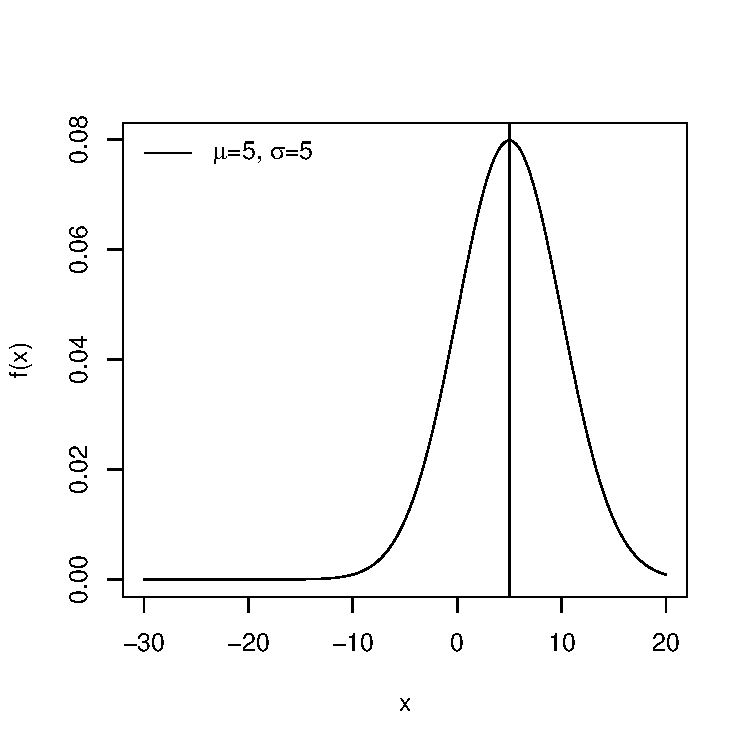
\includegraphics{figure/lec02-003}
\end{center}
\end{frame}
%-------------------------------------------------------------------------------


%-------------------------------------------------------------------------------
\begin{frame}
\frametitle{Normal Example}
\setkeys{Gin}{width=0.7\textwidth}
$\mu$ (mean) specifies the center, $\sigma$ (standard deviation) the spread.
\begin{center}
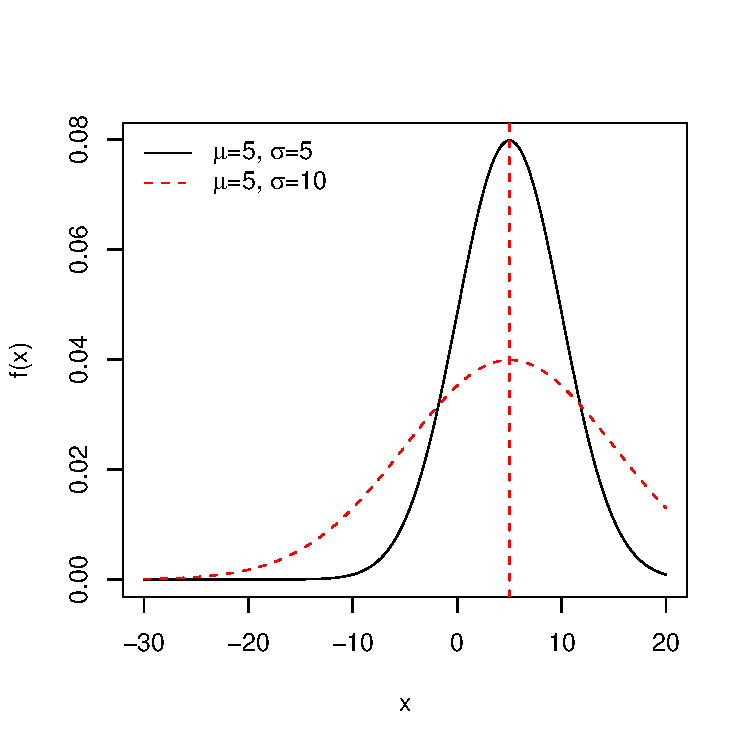
\includegraphics{figure/lec02-004}
\end{center}
\end{frame}
%-------------------------------------------------------------------------------


%-------------------------------------------------------------------------------
\begin{frame}
\frametitle{Normal Example}
\setkeys{Gin}{width=0.7\textwidth}
$\mu$ (mean) specifies the center, $\sigma$ (standard deviation) the spread.
\begin{center}
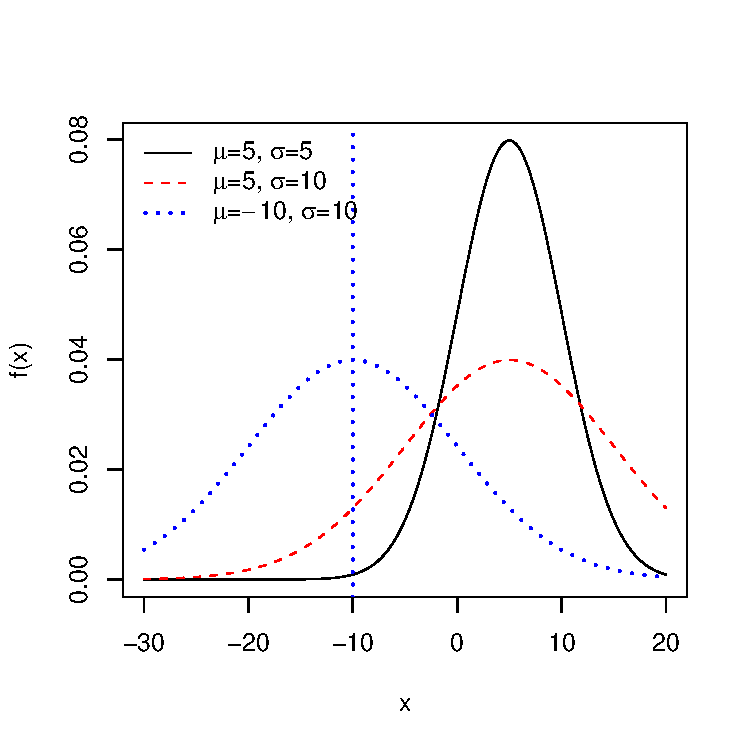
\includegraphics{figure/lec02-005}
\end{center}
\end{frame}
%-------------------------------------------------------------------------------


%pdf("./4.1 Normal Distribution/standard_normal.pdf", height=5, width=5)
%x <- seq(-3.5, 3.5, by=0.01)  
%plot(x,dnorm(x,0,1), type='l', ylab="f(x)", xlab="x")
%dev.off()
%-------------------------------------------------------------------------------
\begin{frame}
\frametitle{Standardized Normal Distribution}
\setkeys{Gin}{width=0.6\textwidth}
If $\mu=0$ and $\sigma=1$, this is the \blue{standard normal distribution}:
\begin{center}
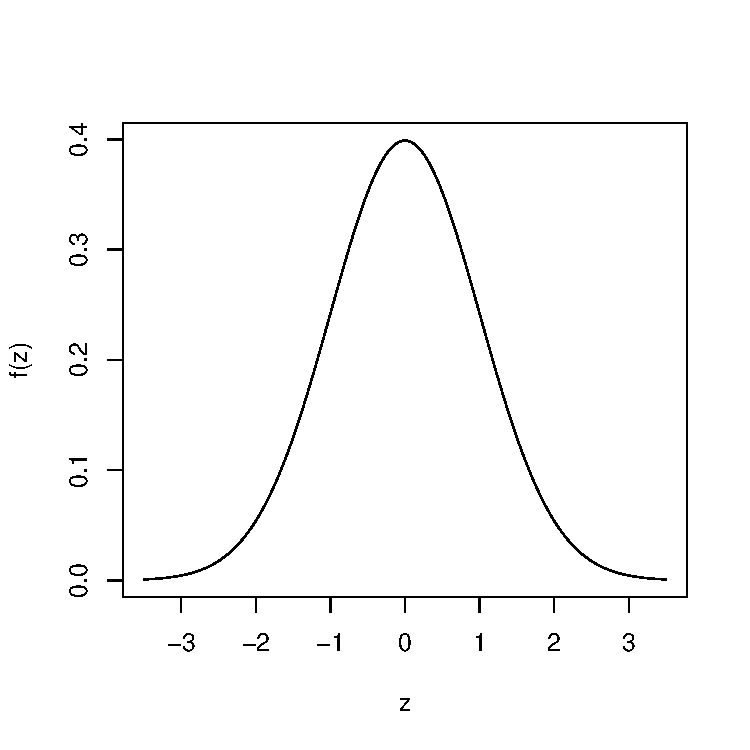
\includegraphics{figure/standard_normal}
\end{center}
\end{frame}
%-------------------------------------------------------------------------------


%-------------------------------------------------------------------------------
\begin{frame}
\frametitle{Rules of Thumb}
Recall if a distribution is normal, then:  
\begin{enumerate}
\item Approx. $\frac{2}{3}$'s of the data are within $\pm 1$ SD of the mean
\item Approx. $95\%$ of the data are within $\pm 2$ SD of the mean
\pause\item Also approx. $99.7\%$ of the data are within $\pm 3$ SD of the mean
\end{enumerate}

\end{frame}
%-------------------------------------------------------------------------------


%-------------------------------------------------------------------------------
\begin{frame}
\frametitle{Ex: Standard Normal $\mu=0$, $\sigma=1$}
\setkeys{Gin}{width=0.75\textwidth}
\begin{center}
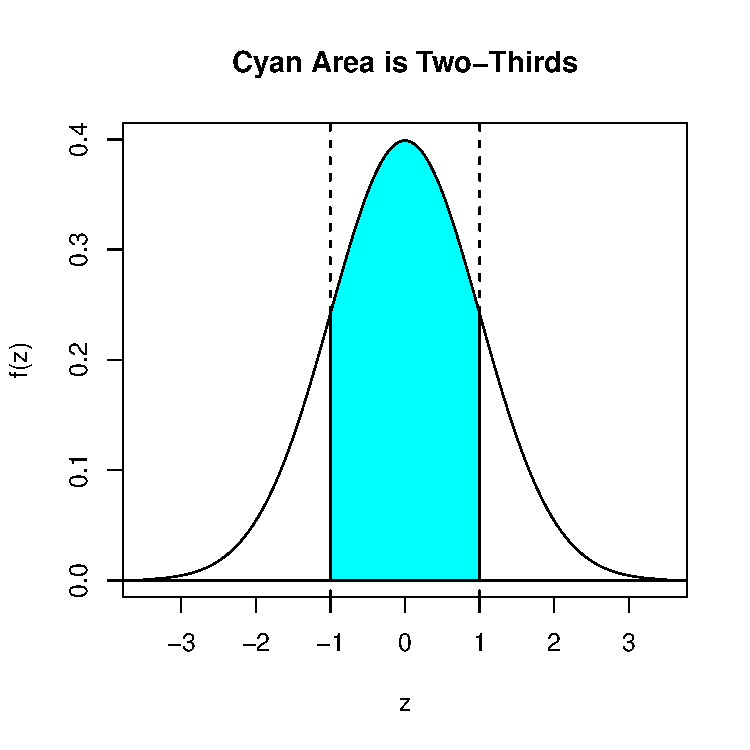
\includegraphics{figure/lec07-001}
\end{center}
\end{frame}
%-------------------------------------------------------------------------------


%-------------------------------------------------------------------------------
\begin{frame}
\frametitle{Ex: Standard Normal $\mu=0$, $\sigma=1$}
\setkeys{Gin}{width=0.75\textwidth}
\begin{center}
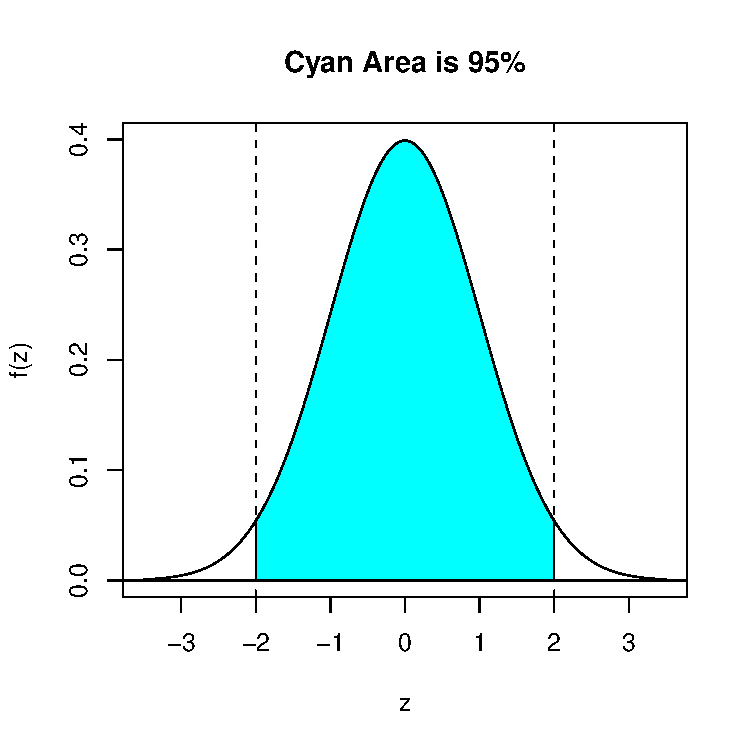
\includegraphics{figure/lec07-002}
\end{center}
\end{frame}
%-------------------------------------------------------------------------------


%-------------------------------------------------------------------------------
\begin{frame}
\frametitle{Ex: Standard Normal $\mu=0$, $\sigma=1$}
\setkeys{Gin}{width=0.75\textwidth}
\begin{center}
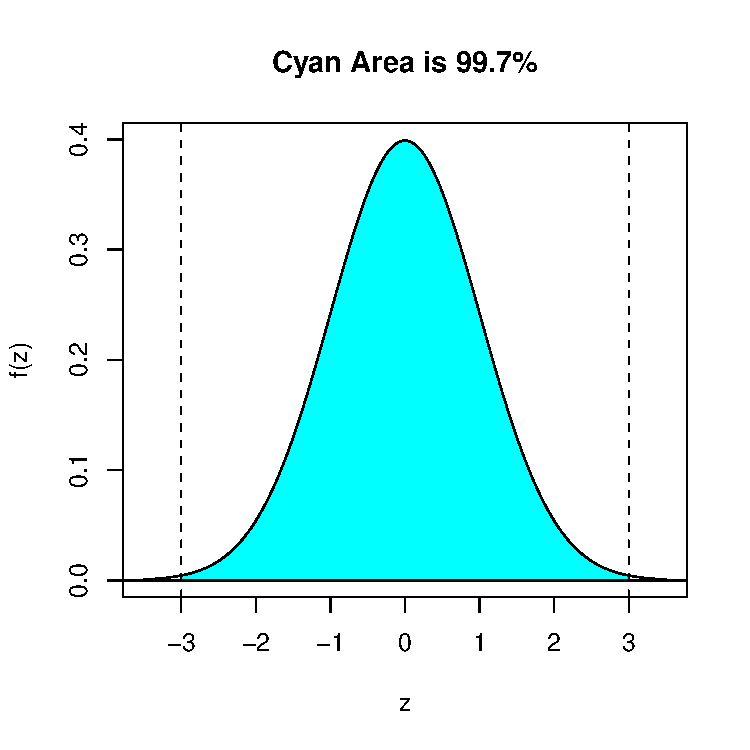
\includegraphics{figure/lec07-003}
\end{center}
\end{frame}
%-------------------------------------------------------------------------------


%-------------------------------------------------------------------------------
\begin{frame}
\frametitle{Motivating Example}
From text:  Say Ann scores 1800 on the SAT and Tom scores 24 on the ACT.  \pause Say both tests scores were normally distributed with:
\begin{small}
\begin{center}
\begin{tabular}{l|rr}
& SAT & ACT \\
\hline
Mean $\mu$ & 1500 & 21\\
SD $\sigma$ & 300 & 5\\
\end{tabular}
\end{center}
\end{small}

\blue{Question}:  Who did relatively better?  


%\vspace{3cm}
%
% Comment this
%
\begin{center}
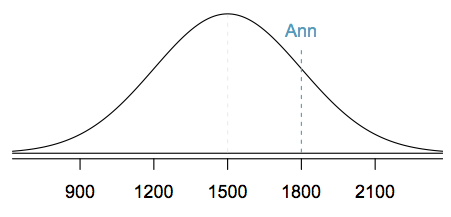
\includegraphics[height=2.5cm]{figure/ann.png}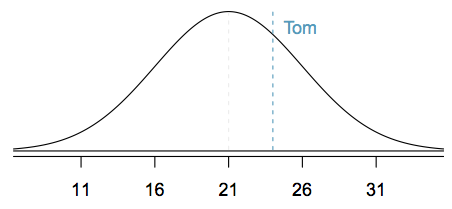
\includegraphics[height=2.5cm]{figure/tom.png}
\end{center}

\end{frame}
%-------------------------------------------------------------------------------


%-------------------------------------------------------------------------------
\begin{frame}
\frametitle{z-scores}
%
% Comment this
%
The \blue{z-score AKA standardized observation} of an observation x is the number of SD it falls above or below the mean. 

\pause\vspace{0.25cm}

The z-score for an observation x that follows a distribution with mean $\mu$ and SD $\sigma$:
\[
z = \frac{x-\mu}{\sigma}
\]

\end{frame}
%-------------------------------------------------------------------------------


%-------------------------------------------------------------------------------
\begin{frame}
\frametitle{z-scores}
%
% Comment this
%
Why is the z-score $z=\frac{x-\mu}{\sigma}$ called the \blue{standardized observation}?  

\begin{enumerate}
\pause\item The observations are \blue{centered} at $\mu$.\\
re-center the $x$ observations to 0 by subtracting $\mu$.
\pause\item The observations have \blue{spread} $\sigma$.\\
re-scale the \blue{spread} of the $x-\mu$ values to be 1 by dividing by $\sigma$.
\end{enumerate}


\pause So we can compare observations from \blue{any} normally distributed data with $(\mu,\sigma)$

\vspace{0.25cm}

\pause i.e. we've \blue{standardized the observations} to make them comparable.
\end{frame}
%-------------------------------------------------------------------------------


%-------------------------------------------------------------------------------
\begin{frame}
\frametitle{Back to Example}
%
% Comment this
%
\begin{itemize}
\item Ann scored 1800. $z=\frac{1800-1500}{300} = +1$ standard deviation from the mean
\item Tom scored 24. $z=\frac{24-21}{5} = +0.6$ standard deviation from the mean
\end{itemize}

So Ann did relatively better.  

\end{frame}
%-------------------------------------------------------------------------------



%-------------------------------------------------------------------------------
\begin{frame}
\frametitle{Percentiles}

Recall a \blue{percentile} (\%'ile) indicates the value below which a given \%'age of observations fall below.

\vspace{0.5cm}

\blue{Question}: What \%'ile is Ann's SAT score of 1800?\\

%
% Comment this
%
i.e. what is the blue shaded area?  
\begin{center}
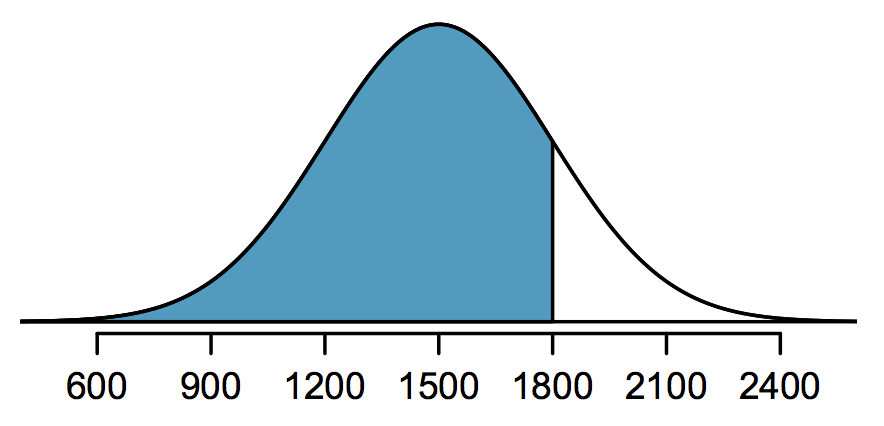
\includegraphics[height=3cm]{figure/ann_z.png}
\end{center}

\end{frame}
%-------------------------------------------------------------------------------






%-------------------------------------------------------------------------------
\begin{frame}
\frametitle{Percentiles}
Because the total area under the curve is 1, the area to the left of z represents the \%'ile of the observation:

\begin{center}
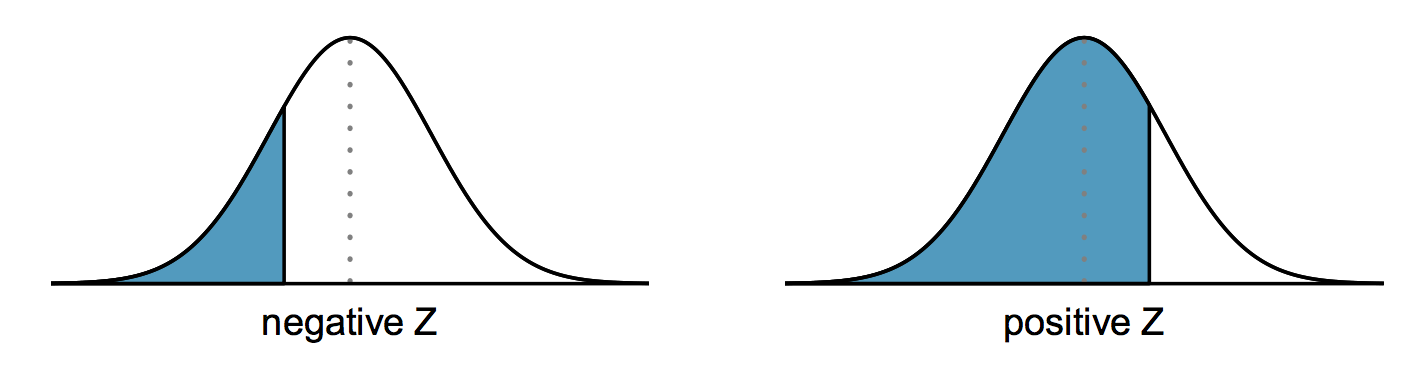
\includegraphics[width=\textwidth]{figure/pos_neg_z.png}
\end{center}

\begin{itemize}
\pause\item The blue shaded area on the left plot will be less than 0.5.  We have \%'iles less than the 50th \%'ile.    
\pause\item The blue shaded area on the right plot will be greater than 0.5.  We have \%'iles greater than the 50th \%'ile.
\end{itemize}

\end{frame}
%-------------------------------------------------------------------------------




%-------------------------------------------------------------------------------
\begin{frame}
\frametitle{Normal Probability Table}

A \blue{normal probability table} allows you to:
\begin{itemize}
\item identify the \%'ile corresponding to a z-score
\item or vice versa: the z-score corresponding to a \%'ile
\end{itemize}

\vspace{0.5cm}

\pause The normal probability tables on page 409 represent z-scores and \%'iles corresponding to area to the left:
\begin{center}
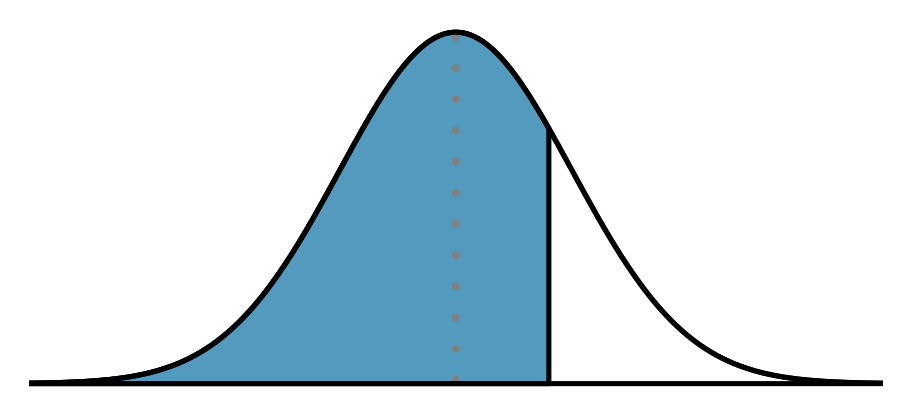
\includegraphics[width=5cm]{figure/area_left.png}
\end{center}

\end{frame}
%-------------------------------------------------------------------------------



%-------------------------------------------------------------------------------
\begin{frame}
\frametitle{Normal Probability Table}
\begin{center}
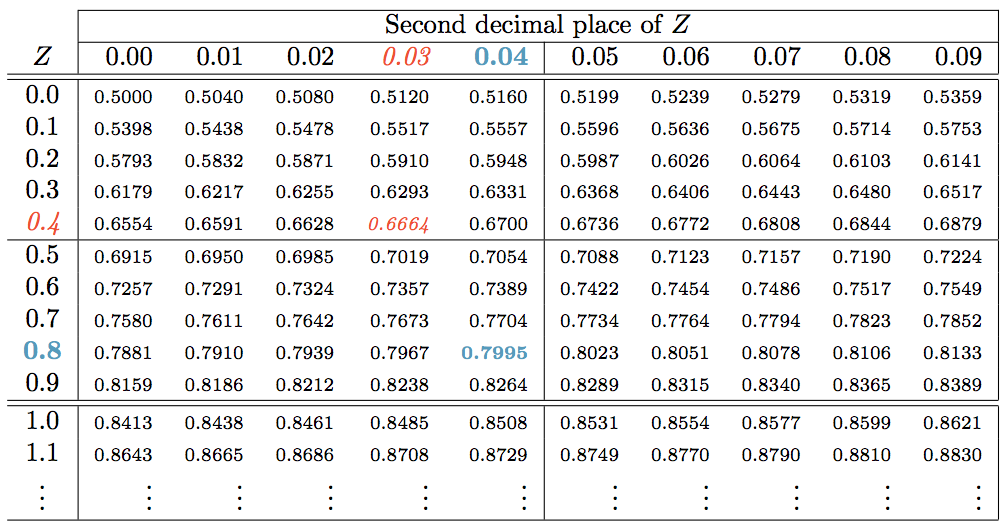
\includegraphics[width=8cm]{figure/normal_table.png}
\end{center}

%
% Comment this
%
\begin{itemize}
\item \textcolor{red}{Red case}: Given a z-score of 0.43.  A lookup tells us the area to the left of z=0.43 is 0.6664, i.e. the 66th \%'ile
\pause\item \textcolor{blue}{Blue case}:  We want the z-score that is the 80th \%'ile.  Reverse lookup: the closest value on the table is 0.7995, i.e. a z-score of 0.84. 
\end{itemize}


\end{frame}
%-------------------------------------------------------------------------------



%-------------------------------------------------------------------------------
\begin{frame}
\frametitle{Back to Ann and Tom}

%
% Comment this
%
\begin{itemize}
\item Since Ann had a z-score of 1.0, her \%'ile is 0.8413. (1.0 row, 0.00 column)\\
i.e. She did better than 84.13\% of SAT test takers.
\pause \item Since Tom had a z-score of 0.6, his \%'ile is 0.7257. (0.6 row, 0.00 column)\\
i.e. He did better than 72.57\% of ACT test takers
\end{itemize}


\end{frame}
%-------------------------------------------------------------------------------





%------------------------------------------------------------------------------
\begin{frame}[fragile]
\frametitle{Next Time}

Next time we will:

\begin{itemize}
\item Re-iterate the motivation for the normal curve.
\item Go over examples using z-scores.
\item Evaluating the normal approximation.
\end{itemize}


\end{frame}
%------------------------------------------------------------------------------







\end{document}










